\chapter{Mapeamento, com identificação e caracterização das áreas de preservação permanente incidentes sobre o imóvel (banhados, cursos d’água, nascentes, reservatórios artificiais de água, lagos, lagoas, topos de morros e montanhas, dunas, locais de refúgio ou reprodução de aves migratórias ou da fauna ameaçada de extinção);}

%\includepdf[pages = {-}, angle = 0, scale = 1]{./anexos/hidro.jpg}

\chapter{Relatório Fotográfico atualizado e representativo do terreno proposto}

%\chapter{Levantamento Planialtimétrico do imóvel proposto, em escala adequada, contendo curvas de nível (isolinhas) equidistantes de 1 metro, demarcando;}
%3.3.1 - Polígono limite do terreno com sistema urbanístico projetado, com aprovação preliminar do orgão competente do município;
\chapter{Recursos hídricos}
\label{chap:hidro}
\clearpage
\includepdf[fitpaper=true]{./anexos/hidrografia.pdf}

%e seus respectivos níveis máximos normais (cotas máximas de inundação/cheia);

\chapter{Áreas de Preservação Permanente (APP)}
\label{chap:rechidr}
\clearpage
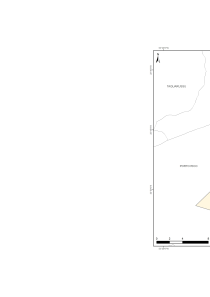
\includepdf[fitpaper=true]{./anexos/app.pdf}

\chapter{Locação, em Planta ou Mapa, dos Pontos onde foram tomadas as fotografias do relatório fotográfico, indicando adireção apontada}
\label{chap:fotografia}
\clearpage

\chapter{Locação, em Planta ou Mapa, dos Pontos dos Testes de Permeabilidade do Solo}
\label{chap:permeabilidade}
\clearpage

\chapter{Locação, em Planta ou Mapa, dos Pontos de Sondagem do Perfil do Solo}
\label{chap:sondspec}
\clearpage
\includepdf[fitpaper=true]{./anexos/sondagens.pdf}
\includepdf[pages = {-}, angle = 0, scale = 1]{./anexos/Relatorio_SPT1.pdf}

\chapter{Mapa de Isodeclividades do relevo}
\label{chap:declividade}
\clearpage
\includepdf[fitpaper=true]{./anexos/isodeclividade.pdf}

\chapter{Aerofoto/Imagem de Satélite com Delimitação da Área Prevista para o Empreendimento}
\label{chap:delimitacao}
\clearpage

\chapter{ANOTAÇÃO DE RESPONSABILIDADE TÉCNICA}
\includepdf[pages = {-}, angle = 0, scale = 0.90]{./anexos/art.pdf}
%ART Todos os documentos (laudos, testes, plantas, levantamentos, informações, etc.) devem ser encaminhados comassinatura do técnico responsável habilitado, constando o nome, qualificação, registro profissional, endereço e telefonepara contato, com emissão de ART devidamente registrada no conselho de classe correspondente.
